\documentclass[12pt]{amsart}
\usepackage[margin=0.5in]{geometry}     
\usepackage[section]{placeins}
\geometry{letterpaper}                   % ... or a4paper or a5paper or ... 
%\geometry{landscape}                % Activate for for rotated page geometry
%\usepackage[parfill]{parskip}    % Activate to begin paragraphs with an empty line rather than an indent
\usepackage{graphicx}
\usepackage{amssymb}
\usepackage{epstopdf}
\DeclareGraphicsRule{.tif}{png}{.png}{`convert #1 `dirname #1`/`basename #1 .tif`.png}


\title{ELEC  243: Lab Report \#1}
\author{Carissa Livingston \& Fernando Ramirez}
\date{\today}




                       % Activate to display a given date or no date

\begin{document}

\maketitle
\section{Summary}
This lab walked us through collecting basic electrical measurements of voltage, resistance, and current using a DMM.  Through the calculations we made we also looked at the mathematical characteristics of wiring circuits both in parallel and series. Additionally we looked at the variance of true resistance between resistors of the same manufactured resistance.  Finally, we examined the equation V=IR to evaluate if it held true for all items with resistive properties, and we found that V=IR is only a valid equation for ohmic resistors; other resistors, such as a light bulbs, photodiode, thermistor, and photocell had resistances that varied due to heat, light, or temperature. The mastery of these ideas will allow us to eventually develop systems of measurement that send varying signals which are determined by measured changes in resistance. The most surprising result from this lab came from our measurements of the light bulb current over several voltages. Knowing the light bulb is not perfectly ohmic we deduced that the it was interesting to see how its relationship of current to voltage varied as the amount of light it produced increased. 


%%%%%%%%%%
\section{Data and Analysis}
\begin{table}[h]
\caption{Battery Voltages} % title of Table
\centering  % used for centering table
\begin{tabular}{c c c c} % centered columns (4 columns)
\hline\hline                        %inserts double horizontal lines
 % inserts table 
%heading
\hline                  % inserts single horizontal line
   Battery & Voltage (V)\\ 
1 & 1.512\\ 
2 & 1.51\\ 
Pack(1+2) & 3.004\\ 
Pack - (1+2) & -0.018  \\ % [1ex] adds vertical space
\hline %inserts single line
\end{tabular}
\label{Measuring Battery Voltages something} % is used to refer this table in the text
\end{table}
%%%%%%%%%%
%%%%%%%%%%
\begin{table}[ht]
\caption{Batch of 10 1 k$\Omega$ Resistors} % title of Table
\centering  % used for centering table
\begin{tabular}{c c c c} % centered columns (4 columns)
\hline\hline                        %inserts double horizontal lines
 % inserts table 
%heading
\hline                  % inserts single horizontal line
Resistor \# & Resistance ($k\Omega$) & \% deviation from 1$k\Omega$\\ 
1 & 988 & 1.2\\ 
2 & 983 & 1.7\\ 
3 & 985 & 1.5\\ 
4 & 987 & 1.3\\ 
5 & 985 & 1.5\\ 
6 & 984 & 1.6\\ 
7 & 993 & 0.7\\ 
8 & 979 & 2.1\\ 
\textbf{9} & \textbf{975} & \textbf{2.5}\\ 
10 & 983 & 1.7\\
% [1ex] adds vertical space
\hline %inserts single line
\end{tabular}
\end{table}
%%%%%%%%%
%%%%%%%%%%
\begin{table}[ht]
\caption{Statistics for Batch of Resistors} % title of Table
\centering  % used for centering table
\begin{tabular}{c c c c} % centered columns (4 columns)
\hline\hline                        %inserts double horizontal lines
 % inserts table 
%heading
\hline                  % inserts single horizontal line
Calculation & ($\Omega$)\\ 
Average & 984.2\\ 
Max-mean & 8.80\\ 
Min-mean & -9.20\\ 
Max Value & 993\\ 
Min Value & 975\\ 
Percent deviation of min value & 2.5\\% [1ex] adds vertical space
\hline %inserts single line
\end{tabular}
\end{table}
%%%%%%%%%%
%%%%%%%%%%
\begin{table}[ht]
\caption{Test of 5 Resistors at Random} % title of Table
\centering  % used for centering table
\begin{tabular}{c c c c} % centered columns (4 columns)
\hline\hline                        %inserts double horizontal lines
 % inserts table 
%heading
\hline                  % inserts single horizontal line
Resistor Colors & Nominal($\Omega$) & Measured($\Omega$)\\ 
br.gr.black & 15 & 14.7\\ 
br.gr.reed & 1500 & 1488\\ 
br.gr.orange & 15000 & 1497\\ 
br.gr.br & 150 & 147.4\\ 
br.black.green & 1000000 & 986000\\% [1ex] adds vertical space
\hline %inserts single line
\end{tabular}
\end{table}
%%%%%%%%%
%%%%%%%%%%
\begin{table}[ht]
\caption{Resistance of the Body: Dry and Wet} % title of Table
\centering  % used for centering table
\begin{tabular}{c c c c} % centered columns (4 columns)
\hline\hline                        %inserts double horizontal lines
 % inserts table 
%heading
\hline                  % inserts single horizontal line
Resistor & Resistance (k$\Omega$)\\ 
Fingers & 550\\ 
Wet Fingers & 100\\% [1ex] adds vertical space
\hline %inserts single line
\end{tabular}
\end{table}
%%%%%%%%%%
%%%%%%%%%%
\begin{table}[ht]
\caption{Deriving Resistance from V \& I} % title of Table
\centering  % used for centering table
\begin{tabular}{c c c c} % centered columns (4 columns)
\hline\hline                        %inserts double horizontal lines
 % inserts table 
%heading
\hline                  % inserts single horizontal line
Voltage(V) & 2.844 & \\ 
Current(mA) & 84.3 & \\ 
Resistance($\Omega$) & 33.73 & Predicted\\ 
Resistance($\Omega$) & 5.2 & Measured\\% [1ex] adds vertical space
\hline %inserts single line
\end{tabular}
\end{table}
%%%%%%%%%%
%%%%%%%%%%
\begin{table}[ht]
\caption{Voltage Supplier Readings} % title of Table
\centering  % used for centering table
\begin{tabular}{c c c c} % centered columns (4 columns)
\hline\hline                        %inserts double horizontal lines
 % inserts table 
%heading
\hline                  % inserts single horizontal line
Power Supply (V) & DMM (V)\\ 
1 & 0.935\\ 
2 & 1.908\\ 
3 & 2.946\\ 
5 & 5.02\\% [1ex] adds vertical space
\hline %inserts single line
\end{tabular}
\end{table}
%%%%%%%%%%
%%%%%%%%%%
\begin{table}[ht]
\caption{Measuring Human R, A, and V} % title of Table
\centering  % used for centering table
\begin{tabular}{c c c c} % centered columns (4 columns)
\hline\hline                        %inserts double horizontal lines
 % inserts table 
%heading
\hline                  % inserts single horizontal line
 Person& Resitance (k$\Omega$) & Current (mA) & Voltage(V)\\ 
Fernando & 500 & 5 & 2500\\ 
Carissa' & 550 & 5 & 2750\\% [1ex] adds vertical space
\hline %inserts single line
\end{tabular}
\label{table:nonlin} % is used to refer this table in the text
\end{table}
%%%%%%%%%%
%%%%%%%%%%
\begin{table}[ht]
\caption{Current over Increments of Voltage} % title of Table
\centering  % used for centering table
\begin{tabular}{c c c c c c} % centered columns (4 columns)
\hline\hline                        %inserts double horizontal lines
 % inserts table 
%heading
\hline                  % inserts single horizontal line
Volts & $I_{lightbulb}$ (mA) & Calculated Resistance & $I_{resistor}$(mA) & Calculated Resistance\\ 
0 & 0.03 & 0.00 & 0 & N/A\\ 
0.05 & 5.92 & 0.01 & 0.01 & 5\\ 
0.1 & 11.56 & 0.01 & 0.01 & 10\\ 
0.15 & 16.79 & 0.01 & 0.02 & 7.5\\ 
0.2 & 27.05 & 0.01 & 0.02 & 10\\ 
0.25 & 26.29 & 0.01 & 0.03 & 8.33\\ 
0.3 & 29.86 & 0.01 & 0.03 & 10\\ 
0.35 & 32.5 & 0.01 & 0.04 & 8.75\\ 
0.4 & 34.3 & 0.01 & 0.04 & 10\\ 
0.45 & 35.8 & 0.01 & 0.05 & 9\\ 
0.5 & 37.5 & 0.01 & 0.05 & 10\\ 
1 & 51.6 & 0.02 & 0.1 & 10\\ 
1.5 & 64.6 & 0.02 & 0.15 & 10\\ 
2 & 74.6 & 0.03 & 0.2 & 10\\ 
2.5 & 84.7 & 0.03 & 0.25 & 10\\ 
3 & 94.5 & 0.03 & 0.3 & 10\\ 
3.5 & 103.7 & 0.03 & 0.35 & 10\\ 
4 & 111.9 & 0.04 & 0.4 & 10\\ 
4.5 & 120 & 0.04 & 0.45 & 10\\ 
5 & 127.7 & 0.04 & 0.5 & 10\\% [1ex] adds vertical space
\hline %inserts single line
\end{tabular}
\end{table}
%%%%%%%%%%

%%%%%%%%%%
\begin{table}[ht]
\caption{Voltage over Circuit Parts} % title of Table
\centering  % used for centering table
\begin{tabular}{c c c c c} % centered columns (4 columns)
\hline\hline                        %inserts double horizontal lines
 % inserts table 
%heading
\hline                  % inserts single horizontal line
$V_{bulb}$ & $V_{batt}$ & $V_{res}$ & $V_{res}-(V_{batt}-V_{bulb})$& $I=V_{res}/R$\\ 
1 & -1.547 & 0.543 & -0.004 & 0.0543\\ 
2 & -2.78 & 0.776 & -0.004 & 0.0776\\ 
3 & -3.97 & 0.968 & -0.002 & 0.0968\\ 
4 & -5.15 & 1.136 & -0.014 & 0.1136\\% [1ex] adds vertical space
\hline %inserts single line
\end{tabular}
\label{table:nonlin} % is used to refer this table in the text
\end{table}
%%%%%%%%%%

%%%%%%%%%%
\begin{table}[ht]
\caption{Measuring Ambient Temperature: Constants and Calculations} % title of Table
\centering  % used for centering table
\begin{tabular}{c c c c c c c} % centered columns (4 columns)
\hline\hline                        %inserts double horizontal lines
 % inserts table 
%heading
\hline                  % inserts single horizontal line
 Environment & Ro & To & B & R & T (K) & T(C)\\ 
Body & 10000 & 298.15 & 4100 & 8200 & 302.52 & 29.37\\ 
Ambient & 10000 & 298.15 & 4100 & 9580 & 299.08 & 25.93\\% [1ex] adds vertical space
\hline %inserts single line
\end{tabular}
\label{table:nonlin} % is used to refer this table in the text
\end{table}
%%%%%%%%%%
%%%%%%%%%%
\begin{table}[ht]
\caption{Photocell Resistance and Photodiode Voltage for several conditions} % title of Table
\centering  % used for centering table
\begin{tabular}{c c c c} % centered columns (4 columns)
\hline\hline                        %inserts double horizontal lines
 % inserts table 
%heading
\hline                  % inserts single horizontal line
  & Photocell &  & Photodiode\\ 
Conditions & Resistance(kohms) & Illumination(lux) & Voltage (V)\\ 
Ambient & 0.577 & 436.24 & 0.321\\ 
shadow & 3.89 & 23.16 & 0.275\\ 
under a hand & 4.7 & 17.31 & 0.015\\ 
iphone light & 0.401 & 763.58 & 0.408\\ 
1ft away from lamp & 0.287 & 1,277.43 & 0.364\\% [1ex] adds vertical space
\hline %inserts single line
\end{tabular}
\end{table}
%%%%%%%%%%
%%%%%%%%%%
\begin{table}[ht]
\caption{Resistance of Photocell over Time} % title of Table
\centering  % used for centering table
\begin{tabular}{c c c c} % centered columns (4 columns)
\hline\hline                        %inserts double horizontal lines
 % inserts table 
%heading
\hline                  % inserts single horizontal line
 Time (s) & Resistance (M$\Omega$)\\ 
10 & 1.6\\ 
20 & 3.66\\ 
30 & 4.75\\ 
40 & 5.59\\ 
50 & 5.49\\ 
60 & 5.61\\% [1ex] adds vertical space
\hline %inserts single line
\end{tabular}
\end{table}
%%%%%%%%%%
%%%%%%%%%%
\begin{table}[ht]
\caption{Diode Current and Voltages in Several Conditions} % title of Table
\centering  % used for centering table
\begin{tabular}{c c c c} % centered columns (4 columns)
\hline\hline                        %inserts double horizontal lines
 % inserts table 
%heading
\hline                  % inserts single horizontal line
 & Diode & \\ 
Conditions & Current (mA) & Voltage (V)\\ 
Ambient & 0.01 & 0.321\\ 
shadow & 0.01 & 0.275\\ 
under a hand & 0.01 & 0.015\\ 
iphone light & 0.01 & 0.408\\ 
1' from lamp & 0.02 & 0.424\\ 
6'' from lamp & 0.05 & 0.458\\ 
3'' from lamp & 0.25 & 0.514\\ 
Directly in front of lamp & 0.32 & 0.55\\% [1ex] adds vertical space
\hline %inserts single line
\end{tabular}
\end{table}
\section{Figures}
\begin{figure}
	\centering
	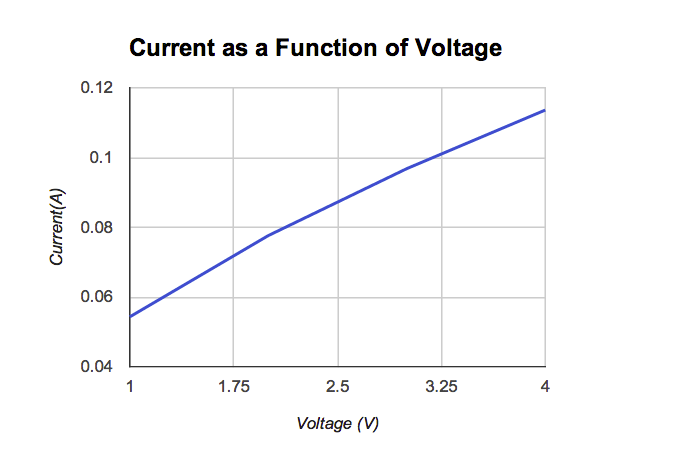
\includegraphics[width=4.2in]{Current}
\end{figure}
\begin{figure}
	\centering
	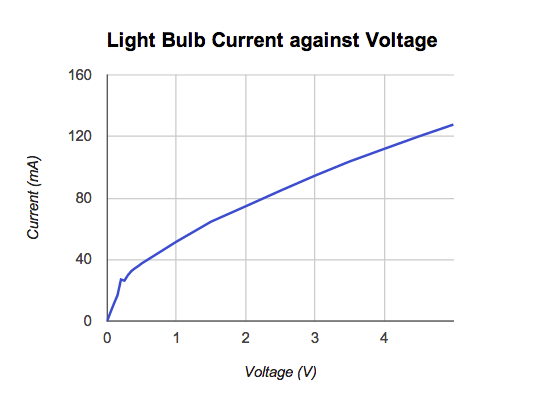
\includegraphics[width=4.2in]{Bulb}
\end{figure}
\begin{figure}
	\centering
	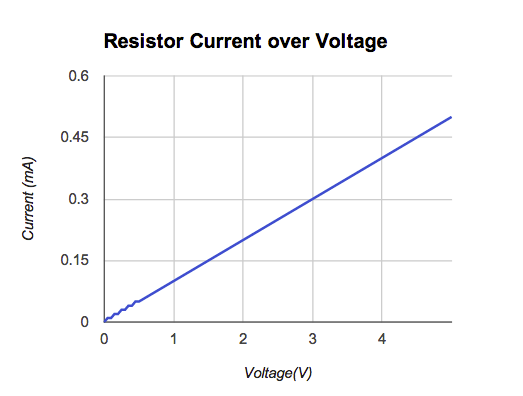
\includegraphics[width=4.2in]{Resistor}
\end{figure}
%%%%%%%%%%\section{DC Measurments with the DMM}

\section{DC Measurments with the DMM}
\noindent Is the measured voltage of the battery pack equal to the sum of the two batteries?\\
\indent The measured voltage of the battery pack, 3.04 Volts, is approximately equal to the sum of the measured individual batteries ($1.512 +1.51 = 3.012 \;\;Volts$).  The small difference is the result of accumulation of errors in measurement.\\ \\
Is the measured battery voltage when connected to the bulb the same as before?  What is the current flowing through the bulb? \\
\indent The measured battery voltage with the light has decreased from 3.004 volts to 2.844 volts. We don't however conclude that the difference in voltage is a direct result of the addition of the light bulb and we suggest it is the result of the measurement being made near the lightbulb, which does not take into account the voltage drop as a result of the resistance in the wires connecting the bulb and the battery pack. In our first measurement we measured near the battery terminal. \\ \\
What's wrong with holding the leads and probes between your fingers when you measure the value of resistors?\\
\indent Holding the leads and probes between fingers when measuring the value of the resistors causes the resistance measurement to increase because the human body acts as a conductor and current travels through it as well as the resistor. \\ \\
\textbf{Question 1:} Formally, the actual resistance $R$ of a resistor having nominal value  and tolerance   lies in the range .  Assuming common nominal and tolerance values, what is the tolerance of a series connection of two such resistors?  Of a parallel connection?  \\
\indent For resistors in Series:
$$R_o(1\pm\delta) + R_o(1\pm\delta) = \Sigma R$$
$$ 2 R_o \pm 2\delta = \Sigma R$$
$$\text{therefore, tolerance is }2\delta$$
\indent For resistors in Series:
$$\frac{1}{R_o(1\pm\delta)} + \frac{1}{R_o(1\pm\delta)} = \frac{1}{R}$$
$$\frac{2}{R_o(1\pm\delta)} = \frac{1}{r}$$
$$ R = \frac{R_o(1\pm\delta)}{2}$$
$$\text{therefore, tolerance is }\frac{1}{2\delta}$$\\
\indent The values shown in Table 2 collected from a batch of 10 resistors exhibits this variability in manufactured resistors.  None of the resistors we measured were out of the tolerance level indicated.\\ \\
\textbf{Question 2:} Calculate the average resistance for your batch of resistors. What is the greatest measured excursion from the mean? Does it lie within the specified tolerance? \\
\indent The average resistance for our batch of resistors was 984.2 $\Omega$ withthe greatest measured excursion from the mean being the min value of the group which is 975 $\Omega$ with 2.5\% excursion from the nominal value of 1 $k\Omega$ which is within the 5\% tolerance indicated by the gold band of the resistors(Table 3)\\ \\
\textbf{Question 3:} How do we know which is more nearly correct: the DMM or the labels on the resistors?
\indent The DMM is more nearly correct because it is a live measure of the resistor while the manufacturer's markings are only meant to indicate the general resistance range that the resistor operates in for purposes of quality control within large scale manufacturing.\\ \\
Based on the resistance measurements you made with your DMM, what is the resolution of your resistance measurements? 
\indent The resolution of our measurements is about 100,000 Mohms\\ \\
When you measure your body resistance, does your resistance change when you wet your fingers? If so, speculate why. Calculate what voltage would be necessary to produce a 5 mA current through you. Why is 5 mA significant?\\
\indent Yes, when we measured initial resistance the body varied between $.55-65 \;M\Omega$. The resistance of the wet skin was significantly less than that of the dry, approximately $100\;k\Omega$. This is because adding a liquid with ions, in this case saliva with several electrolytes, increases the conductivity and reduces resistance(Table 5).\\ \\
Using the DMM, measure the resistance of the light bulb. Does this correspond to the value you would expect from Ohm's Law given the values of voltage and current you measured in Parts 1 and 2?\\
\indent The DMM measured resistance of our light bulb was $5.2 \Omega$. Using Ohms law with a voltage of 2.844 V and a current of 84.3 mAmps the expected resistance is 33.73 $\Omega$. The values do not correspond. They do not correspond because the light bulb is not ohmic, implying that its resistance does not vary directly with the voltage. A light bulb's resistance increases with temperature, meaning that the expected resistance, calculated when voltage is applied and current is flowing through the bulb, will be higher than the resistance measured when the bulb is not heated and not being supplied with a current.
\indent Table 7 sums up our comparison in voltage readings between the power supply and the DMM.  The DMM has a higher resolution than the Power Supply and as a result will be used to make measurements of voltage.\\ \\
%%%%%%%%%%%%%%%%%%%%%%%%%%%5%%%%%%%%%%%%%%%%%%%%%%
%Bulb

%%%%%%%%%%%%%%%%%%%%%%%%%%%%%%%%%%%%%%%%%%%%%%%%%
\textbf{Question 4}: To what point on this curve does the value of resistance you measured with the ohmmeter correspond?\\
\indent Referring to Figure 1 it can be seen by dividing each current by the corresponding voltage we get the inverse of the resistance.  This goes to say that the inverse of resistance is the slope of the graphed line. The point on the curve that our resistance corresponds with was found using an excel equation to match the data. $$y = -315.37x_2 + 378.23x_1 + 13.122 \text{ and } x/y = 5.2$$ $$\text{yielded the solution:}$$ $$\text{Volts}\;=\;1.23247 \;V,   \text{Current}\;=\;0.237014\;A$$.\\
Is our assumption that I = V/R for all V a valid one?\\
\indent No, our assumption that V = IR holds valid for the 1000 ohm resistor as is seen by the linear graph; however, V=IR is not valid for the graph of the light bulb volts and current as seen by the non linear graph that is produced. 
Table 10 Shows that the sum of the voltage drops over the two resistors( the lightbulb and the 10 $\Omega$ resistor) is equal to the voltage drop across the battery.
%%%%%%%%%%%%%%%%%%%%%%%%%%%5%%%%%%%%%%%%%%%%%%%%%%
%Resistor

%Other
%%%%%%%%%%%%%%%%%%%%%%%%%%%%%%%%%%%%%%%%%%%%%%%%%
\section{Measuring Heat and Light}
Table 11 sums up the measurements of resistance of ambient and body temperature and the calculations used to derive the bodily and ambient temperatures.  
This was calculated using the governing equation for the thermistor $$R = R_oe^{B(\frac{1}{T}-\frac{1}{T_o})}$$ and the given value of $$ B = 4100 k \text{ for our } 10 k\Omega\;\text{at}\; 25^{o}C$$
There fore using the governing equation with the given constants we specify
$$R = 10000e^{4100(\frac{1}{T}-\frac{1}{25+273.15})}$$
and find that when  $R =9.58 k\Omega$, temperature is 299K (78 degrees F), and when in contact with a body $R =8.20 k\Omega$, and temperature is 302K (84 degrees F). Though the body temperature was found to be slightly lower than expected body temperature, our thermistor was placed between two fingers to measure core body temperature. A more accurate reading for body temperature would have been to place the thermistor in someone�s mount, or under their arm. However, because we did not wish to break the thermistor, this was not done, and a lower temperature was expected. 
Tables 12 and14 sum up the measurements made in different conditions for the photocell and photodiode.\\
Using the nominal values of the photocell, and deriving the following equation from its log graph,
$$log(R)= mlog(Ill) + B$$
Taking that $$B = log(30)$$
and $$m = -.65$$ we derived an equation to solve for illuminance
$$Ill = R^{\frac{1}{m}}10^{\frac{-B}{m}}=R^{-\frac{1}{-.65}}10^{\frac{-log(30)}{.65}}.$$
Using this equation the illumination in the lab was determined to be 436.24 Lux, consistent with the range for office illuminecense of 400-520 Lux, and that of a foot from the lamp to be 1277 Lux.   
Table 13 sums up our measurements for the increasing resistance of a photodiode in darkness over time.  The value for resistance became stable at approximately 50 seconds.  
Similarly to how the equation for illumination was derived for the photocell, the equation for illumination as a function of current was derived for the photodiode.  The slope was calculated with the data points (300,2) and (30,.02)
$$m = \frac{log(2)-log(.02)}{log(300)-log(30)}= 1$$
and b using the the data points (300,2) and the equation
$$log(i)= mlog(Ill) + B$$
to be  
$$B = -2.17.$$
With m, B, and the following equation for Ill. The ambient illumination and the illumination 1' from the lamp were determined to be 1479 lx and 47331 lx respectively.
$$Ill = i^{\frac{1}{m}}10^{\frac{-B}{m}}=i^{-\frac{1}{1}}10^{\frac{-2.17}{1}}.$$
These values are not exactly in the same relative area as each other but the trend of the light having a higher lx value was consistent.  The error in measuring could have come from measuring such small currents through the circuit and the lack of accuracy in the diode itself.  It ca be seen in Table 14 that rounding error played a big part with the current only reaching a percent of a mA for most environments.

\section{Feedback}
This lab was very straightforward and was also very useful to help reorient us with basic electronic measurement devices; we cannot think of anything that could be improved upon in the lab material however having to wait to ask a group to use their DMM device was rather annoying and if that can be redone in anyway would be very nice.

\end{document}  